\documentclass{beamer}

% Should be documentclass beamer

\mode<presentation>
{
%  \usetheme[hideothersubsections]{PaloAlto}
  \usetheme{metropolis}
  \setbeamercovered{transparent}
}

\usepackage{amsfonts}
\usepackage{amsmath}
\usepackage{amssymb}
\usepackage{color}
\usepackage{tikz}
\usepackage{pgfplots}
\usepackage{listings}
\usepackage{courier}
%\usepackage[utf8]{inputenc}
%\usepackage[russian]{babel}

\lstset{
  numbers=left,
  basicstyle=\ttfamily\footnotesize,
  numberstyle=\tiny\color{gray},
  stepnumber=1,
  numbersep=10pt,
}

\newcommand{\iu}{\ensuremath{\mathrm{i}}}
\newcommand{\bbR}{\mathbb{R}}
\newcommand{\bbC}{\mathbb{C}}
\newcommand{\calV}{\mathcal{V}}
\newcommand{\calW}{\mathcal{W}}
\newcommand{\macheps}{\epsilon_{\mathrm{mach}}}
\newcommand{\matlab}{\textsc{Matlab}}

\newcommand{\ddiag}{\operatorname{diag}}
\newcommand{\fl}{\operatorname{fl}}
\newcommand{\nnz}{\operatorname{nnz}}
\newcommand{\tr}{\operatorname{tr}}
\renewcommand{\vec}{\operatorname{vec}}

\newcommand{\vertiii}[1]{{\left\vert\kern-0.25ex\left\vert\kern-0.25ex\left\vert #1
    \right\vert\kern-0.25ex\right\vert\kern-0.25ex\right\vert}}
\newcommand{\ip}[2]{\langle #1, #2 \rangle}
\newcommand{\ipx}[2]{\left\langle #1, #2 \right\rangle}
\newcommand{\order}[1]{O( #1 )}

\newcommand{\kron}{\otimes}


\newcommand{\hdr}[2]{
  \title[CS 5220, Fall 2017]{CS 5220: #2}
  \author{David Bindel}
  \date{#1}
}


\hdr{2017-09-19}{Distributed Memory Programming}

\begin{document}

\begin{frame}
  \titlepage
\end{frame}


\begin{frame}
  \frametitle{Plan for this week}

  \begin{itemize}
  \item This week: distributed memory programming
    \begin{itemize}
    \item Distributed memory HW issues (topologies, cost models)
    \item Message-passing programming concepts (and MPI)
    \item Some simple examples
    \end{itemize}

  \vspace{5mm}
  \item Next week: shared memory programming
    \begin{itemize}
    \item Shared memory HW issues (cache coherence)
    \item Threaded programming concepts (pthreads and OpenMP)
    \item A simple example (Monte Carlo)
    \end{itemize}
  \end{itemize}
    
\end{frame}


\begin{frame}
  \frametitle{Basic questions}

  How much does a message cost?
  \begin{itemize}
  \item {\em Latency}: time to get between processors
  \item {\em Bandwidth}: data transferred per unit time
  \item How does {\em contention} affect communication?
  \end{itemize}
  This is a combined hardware-software question!

  \vspace{5mm}
  We want to understand just enough for reasonable modeling.

\end{frame}


\begin{frame}
  \frametitle{Thinking about interconnects}

  Several features characterize an interconnect:
  \begin{itemize}
  \item {\em Topology}: who do the wires connect?
  \item {\em Routing}: how do we get from A to B?
  \item {\em Switching}: circuits, store-and-forward?
  \item {\em Flow control}: how do we manage limited resources?
  \end{itemize}
\end{frame}


\begin{frame}
  \frametitle{Thinking about interconnects}

  \begin{itemize}
  \item Links are like streets
  \item Switches are like intersections
  \item Hops are like blocks traveled
  \item Routing algorithm is like a travel plan
  \item Stop lights are like flow control
  \item Short packets are like cars,
    long ones like buses?
  \end{itemize}
  At some point the analogy breaks down...

\end{frame}


\begin{frame}
  \frametitle{Bus topology}

  \begin{center}
    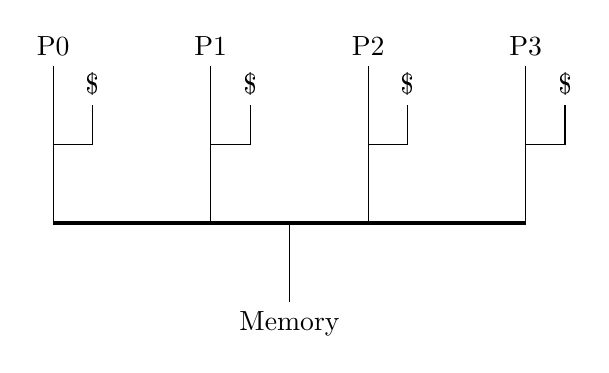
\begin{tikzpicture}
\draw[ultra thick] (0,0) -- (6,0);
\draw (3,0) -- (3,-1) node[below] {Memory};
\draw (0,0) -- (0,2) node[above] {P0};
\draw (0,1) -- (0.5,1) -- (0.5,1.5) node[above]{\$};
\draw (2,0) -- (2,2) node[above] {P1};
\draw (2,1) -- (2.5,1) -- (2.5,1.5) node[above]{\$};
\draw (4,0) -- (4,2) node[above] {P2};
\draw (4,1) -- (4.5,1) -- (4.5,1.5) node[above]{\$};
\draw (6,0) -- (6,2) node[above] {P3};
\draw (6,1) -- (6.5,1) -- (6.5,1.5) node[above]{\$};
\end{tikzpicture}

  \end{center}

  \begin{itemize}
  \item One set of wires (the bus)
  \item Only one processor allowed at any given time
    \begin{itemize}
    \item {\em Contention} for the bus is an issue
    \end{itemize}
  \item Example: basic Ethernet, some SMPs
  \end{itemize}

\end{frame}


\begin{frame}
  \frametitle{Crossbar}

  \begin{center}
    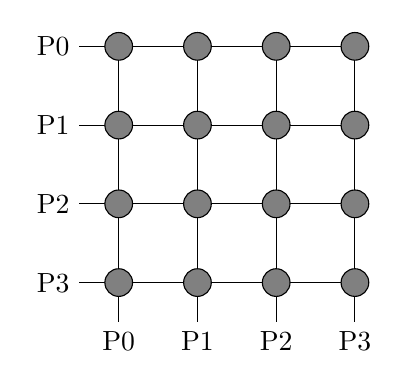
\begin{tikzpicture}
% Horizontal lines
\draw (-0.5,0) node[left] {P3} -- (3,0);
\draw (-0.5,1) node[left] {P2} -- (3,1);
\draw (-0.5,2) node[left] {P1} -- (3,2);
\draw (-0.5,3) node[left] {P0} -- (3,3);
% Vertical lines
\draw (0,-0.5) node[below] {P0} -- (0,3);
\draw (1,-0.5) node[below] {P1} -- (1,3);
\draw (2,-0.5) node[below] {P2} -- (2,3);
\draw (3,-0.5) node[below] {P3} -- (3,3);
% Intersection circles
\draw[fill=black!50] (0,0) circle (5pt);
\draw[fill=black!50] (0,1) circle (5pt);
\draw[fill=black!50] (0,2) circle (5pt);
\draw[fill=black!50] (0,3) circle (5pt);
\draw[fill=black!50] (1,0) circle (5pt);
\draw[fill=black!50] (1,1) circle (5pt);
\draw[fill=black!50] (1,2) circle (5pt);
\draw[fill=black!50] (1,3) circle (5pt);
\draw[fill=black!50] (2,0) circle (5pt);
\draw[fill=black!50] (2,1) circle (5pt);
\draw[fill=black!50] (2,2) circle (5pt);
\draw[fill=black!50] (2,3) circle (5pt);
\draw[fill=black!50] (3,0) circle (5pt);
\draw[fill=black!50] (3,1) circle (5pt);
\draw[fill=black!50] (3,2) circle (5pt);
\draw[fill=black!50] (3,3) circle (5pt);
\end{tikzpicture}

  \end{center}

  \begin{itemize}
  \item Dedicated path from every input to every output
    \begin{itemize}
    \item Takes $O(p^2)$ switches and wires!
    \end{itemize}
  \item Example: recent AMD/Intel multicore chips \\
    (older: front-side bus)
  \end{itemize}

\end{frame}


\begin{frame}
  \frametitle{Bus vs. crossbar}

  \begin{itemize}
  \item Crossbar: more hardware
  \item Bus: more contention (less capacity?)
  \item Generally seek happy medium
    \begin{itemize}
    \item Less contention than bus
    \item Less hardware than crossbar
    \item May give up one-hop routing
    \end{itemize}
  \end{itemize}
\end{frame}


\begin{frame}
  \frametitle{Network properties}
  
  Think about latency and bandwidth via two quantities:
  \begin{itemize}
  \item {\em Diameter}: max distance between nodes
  \item {\em Bisection bandwidth}: smallest bandwidth cut to bisect
    \begin{itemize}
    \item Particularly important for all-to-all communication
    \end{itemize}
  \end{itemize}
  
\end{frame}


\begin{frame}
  \frametitle{Linear topology}
  
  \begin{center}
  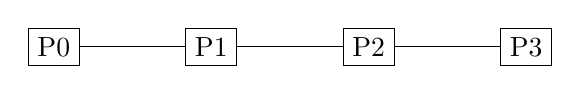
\begin{tikzpicture}
\node (lt0) [draw,rectangle] at (0,0) {P0};
\node (lt1) [draw,rectangle] at (2,0) {P1};
\node (lt2) [draw,rectangle] at (4,0) {P2};
\node (lt3) [draw,rectangle] at (6,0) {P3};
\draw (lt0) -- (lt1);
\draw (lt1) -- (lt2);
\draw (lt2) -- (lt3);
\end{tikzpicture}

  \end{center}
  \begin{itemize}
  \item $p-1$ links
  \item Diameter $p-1$
  \item Bisection bandwidth $1$
  \end{itemize}
\end{frame}


\begin{frame}
  \frametitle{Ring topology}

  \begin{center}
  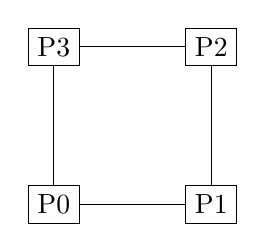
\begin{tikzpicture}
\node (lt0) [draw,rectangle] at (0,0) {P0};
\node (lt1) [draw,rectangle] at (2,0) {P1};
\node (lt2) [draw,rectangle] at (2,2) {P2};
\node (lt3) [draw,rectangle] at (0,2) {P3};
\draw (lt0) -- (lt1);
\draw (lt1) -- (lt2);
\draw (lt2) -- (lt3);
\draw (lt3) -- (lt0);
\end{tikzpicture}

  \end{center}

  \begin{itemize}
  \item $p$ links
  \item Diameter $p/2$
  \item Bisection bandwidth $2$
  \end{itemize}

\end{frame}


\begin{frame}
  \frametitle{Mesh}

  \begin{center}
  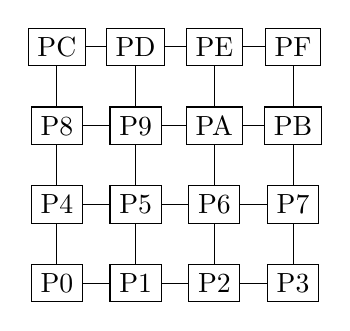
\begin{tikzpicture}
\node (mt0) [draw,rectangle] at (0,0) {P0};
\node (mt1) [draw,rectangle] at (1,0) {P1};
\node (mt2) [draw,rectangle] at (2,0) {P2};
\node (mt3) [draw,rectangle] at (3,0) {P3};
\node (mt4) [draw,rectangle] at (0,1) {P4};
\node (mt5) [draw,rectangle] at (1,1) {P5};
\node (mt6) [draw,rectangle] at (2,1) {P6};
\node (mt7) [draw,rectangle] at (3,1) {P7};
\node (mt8) [draw,rectangle] at (0,2) {P8};
\node (mt9) [draw,rectangle] at (1,2) {P9};
\node (mtA) [draw,rectangle] at (2,2) {PA};
\node (mtB) [draw,rectangle] at (3,2) {PB};
\node (mtC) [draw,rectangle] at (0,3) {PC};
\node (mtD) [draw,rectangle] at (1,3) {PD};
\node (mtE) [draw,rectangle] at (2,3) {PE};
\node (mtF) [draw,rectangle] at (3,3) {PF};

\draw (mt0) -- (mt1);  \draw (mt0) -- (mt4);
\draw (mt1) -- (mt2);  \draw (mt4) -- (mt8);
\draw (mt2) -- (mt3);  \draw (mt8) -- (mtC);

\draw (mt4) -- (mt5);  \draw (mt1) -- (mt5);
\draw (mt5) -- (mt6);  \draw (mt5) -- (mt9);
\draw (mt6) -- (mt7);  \draw (mt9) -- (mtD);

\draw (mt8) -- (mt9);  \draw (mt2) -- (mt6);
\draw (mt9) -- (mtA);  \draw (mt6) -- (mtA);
\draw (mtA) -- (mtB);  \draw (mtA) -- (mtE);

\draw (mtC) -- (mtD);  \draw (mt3) -- (mt7);
\draw (mtD) -- (mtE);  \draw (mt7) -- (mtB);
\draw (mtE) -- (mtF);  \draw (mtB) -- (mtF);

\end{tikzpicture}

  \end{center}
  \begin{itemize}
  \item May be more than two dimensions
  \item Route along each dimension in turn
  \end{itemize}
\end{frame}


\begin{frame}
  \frametitle{Torus}

  \begin{center}
    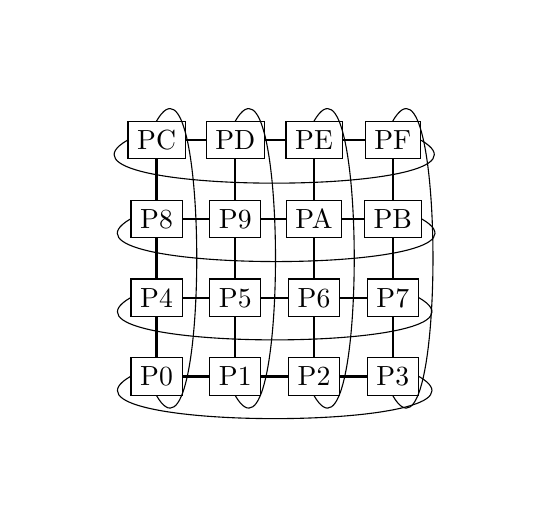
\begin{tikzpicture}
\node (mt0) [draw,rectangle] at (0,0) {P0};
\node (mt1) [draw,rectangle] at (1,0) {P1};
\node (mt2) [draw,rectangle] at (2,0) {P2};
\node (mt3) [draw,rectangle] at (3,0) {P3};
\node (mt4) [draw,rectangle] at (0,1) {P4};
\node (mt5) [draw,rectangle] at (1,1) {P5};
\node (mt6) [draw,rectangle] at (2,1) {P6};
\node (mt7) [draw,rectangle] at (3,1) {P7};
\node (mt8) [draw,rectangle] at (0,2) {P8};
\node (mt9) [draw,rectangle] at (1,2) {P9};
\node (mtA) [draw,rectangle] at (2,2) {PA};
\node (mtB) [draw,rectangle] at (3,2) {PB};
\node (mtC) [draw,rectangle] at (0,3) {PC};
\node (mtD) [draw,rectangle] at (1,3) {PD};
\node (mtE) [draw,rectangle] at (2,3) {PE};
\node (mtF) [draw,rectangle] at (3,3) {PF};

\draw[thick] (mt0) -- (mt1);  \draw[thick] (mt0) -- (mt4);
\draw[thick] (mt1) -- (mt2);  \draw[thick] (mt4) -- (mt8);
\draw[thick] (mt2) -- (mt3);  \draw[thick] (mt8) -- (mtC);
\draw (mt3.east) to[out=-30,in=210] (mt0.west);
\draw (mtC.north) to[out=60,in=-60] (mt0.south);

\draw[thick] (mt4) -- (mt5);  \draw[thick] (mt1) -- (mt5);
\draw[thick] (mt5) -- (mt6);  \draw[thick] (mt5) -- (mt9);
\draw[thick] (mt6) -- (mt7);  \draw[thick] (mt9) -- (mtD);
\draw (mt7.east) to[out=-30,in=210] (mt4.west);
\draw (mtD.north) to[out=60,in=-60] (mt1.south);

\draw[thick] (mt8) -- (mt9);  \draw[thick] (mt2) -- (mt6);
\draw[thick] (mt9) -- (mtA);  \draw[thick] (mt6) -- (mtA);
\draw[thick] (mtA) -- (mtB);  \draw[thick] (mtA) -- (mtE);
\draw (mtB.east) to[out=-30,in=210] (mt8.west);
\draw (mtE.north) to[out=60,in=-60] (mt2.south);

\draw[thick] (mtC) -- (mtD);  \draw[thick] (mt3) -- (mt7);
\draw[thick] (mtD) -- (mtE);  \draw[thick] (mt7) -- (mtB);
\draw[thick] (mtE) -- (mtF);  \draw[thick] (mtB) -- (mtF);
\draw (mtF.east) to[out=-30,in=210] (mtC.west);
\draw (mtF.north) to[out=60,in=-60] (mt3.south);

\end{tikzpicture} \\
    Torus : Mesh :: Ring : Linear
  \end{center}
\end{frame}


\begin{frame}
  \frametitle{Hypercube}
  \begin{center}
  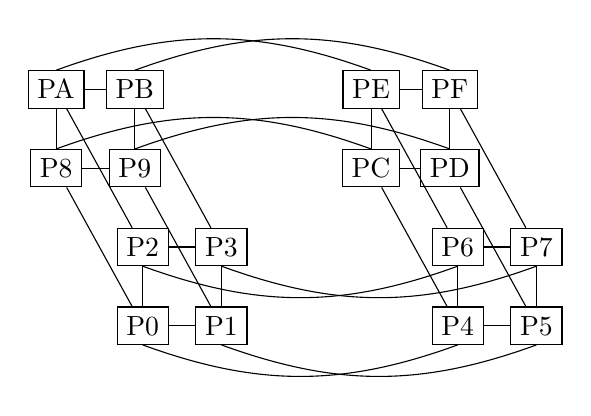
\begin{tikzpicture}
\node (ht0) [draw,rectangle] at (0,0) {P0};
\node (ht1) [draw,rectangle] at (1,0) {P1};
\node (ht2) [draw,rectangle] at (0,1) {P2};
\node (ht3) [draw,rectangle] at (1,1) {P3};

\begin{scope}[xshift=4cm]
\node (ht4) [draw,rectangle] at (0,0) {P4};
\node (ht5) [draw,rectangle] at (1,0) {P5};
\node (ht6) [draw,rectangle] at (0,1) {P6};
\node (ht7) [draw,rectangle] at (1,1) {P7};
\end{scope}

\begin{scope}[yshift=2cm,xshift=-1.1cm]]
\node (ht8) [draw,rectangle] at (0,0) {P8};
\node (ht9) [draw,rectangle] at (1,0) {P9};
\node (htA) [draw,rectangle] at (0,1) {PA};
\node (htB) [draw,rectangle] at (1,1) {PB};

\begin{scope}[xshift=4cm]
\node (htC) [draw,rectangle] at (0,0) {PC};
\node (htD) [draw,rectangle] at (1,0) {PD};
\node (htE) [draw,rectangle] at (0,1) {PE};
\node (htF) [draw,rectangle] at (1,1) {PF};
\end{scope}
\end{scope}

\draw (ht0) -- (ht1);
\draw (ht0) -- (ht2);
\draw (ht2) -- (ht3);
\draw (ht1) -- (ht3);

\draw (ht4) -- (ht5);
\draw (ht4) -- (ht6);
\draw (ht6) -- (ht7);
\draw (ht5) -- (ht7);

\draw (ht0.south) to[out=-20,in=-160] (ht4.south);
\draw (ht1.south) to[out=-20,in=-160] (ht5.south);
\draw (ht2.south) to[out=-20,in=-160] (ht6.south);
\draw (ht3.south) to[out=-20,in=-160] (ht7.south);

\draw (ht8) -- (ht9);
\draw (ht8) -- (htA);
\draw (htA) -- (htB);
\draw (ht9) -- (htB);

\draw (htC) -- (htD);
\draw (htC) -- (htE);
\draw (htE) -- (htF);
\draw (htD) -- (htF);

\draw (ht8.north) to[out=20,in=160] (htC.north);
\draw (ht9.north) to[out=20,in=160] (htD.north);
\draw (htA.north) to[out=20,in=160] (htE.north);
\draw (htB.north) to[out=20,in=160] (htF.north);

\draw (ht0) -- (ht8);
\draw (ht1) -- (ht9);
\draw (ht2) -- (htA);
\draw (ht3) -- (htB);

\draw (ht4) -- (htC);
\draw (ht5) -- (htD);
\draw (ht6) -- (htE);
\draw (ht7) -- (htF);

\end{tikzpicture}

  \end{center}
  \begin{itemize}
  \item Label processors with binary numbers
  \item Connect $p_1$ to $p_2$ if labels differ in one bit
  \end{itemize}
\end{frame}


\begin{frame}
  \frametitle{Fat tree}
  \begin{center}
  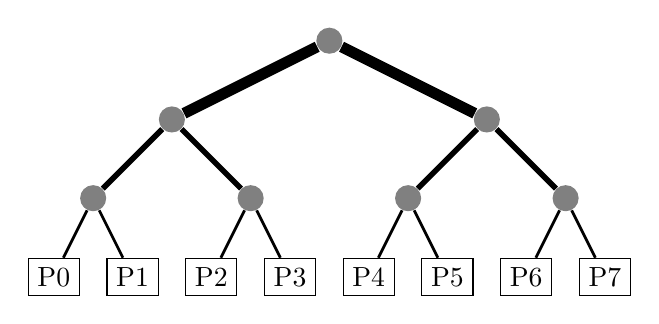
\begin{tikzpicture}
\node(ft0) [draw,rectangle] at (0,0) {P0};
\node(ft1) [draw,rectangle] at (1,0) {P1};
\node(ft2) [draw,rectangle] at (2,0) {P2};
\node(ft3) [draw,rectangle] at (3,0) {P3};
\node(ft4) [draw,rectangle] at (4,0) {P4};
\node(ft5) [draw,rectangle] at (5,0) {P5};
\node(ft6) [draw,rectangle] at (6,0) {P6};
\node(ft7) [draw,rectangle] at (7,0) {P7};

\node(ft01) [circle,fill=black!50] at (0.5,1) { };
\node(ft23) [circle,fill=black!50] at (2.5,1) { };
\node(ft45) [circle,fill=black!50] at (4.5,1) { };
\node(ft67) [circle,fill=black!50] at (6.5,1) { };

\node(ft03) [circle,fill=black!50] at (1.5,2) { };
\node(ft47) [circle,fill=black!50] at (5.5,2) { };

\node(ft07) [circle,fill=black!50] at (3.5,3) { };

\draw[line width=1pt] (ft0) -- (ft01);
\draw[line width=1pt] (ft1) -- (ft01);
\draw[line width=1pt] (ft2) -- (ft23);
\draw[line width=1pt] (ft3) -- (ft23);
\draw[line width=1pt] (ft4) -- (ft45);
\draw[line width=1pt] (ft5) -- (ft45);
\draw[line width=1pt] (ft6) -- (ft67);
\draw[line width=1pt] (ft7) -- (ft67);

\draw[line width=2pt] (ft01) -- (ft03);
\draw[line width=2pt] (ft23) -- (ft03);
\draw[line width=2pt] (ft45) -- (ft47);
\draw[line width=2pt] (ft67) -- (ft47);

\draw[line width=4pt] (ft03) -- (ft07);
\draw[line width=4pt] (ft47) -- (ft07);

\end{tikzpicture}

  \end{center}
  \begin{itemize}
  \item Processors at leaves
  \item Increase link bandwidth near root
  \end{itemize}
\end{frame}


\begin{frame}
  \frametitle{Others...}

  \begin{itemize}
  \item Butterfly network
  \item Omega network
  \item Cayley graph
  \end{itemize}
\end{frame}


\begin{frame}
  \frametitle{Current picture}

  \begin{itemize}
  \item Old: latencies = hops
  \item New: roughly constant latency (?)
    \begin{itemize}
    \item Wormhole routing (or cut-through) flattens latencies
      vs store-forward at hardware level
    \item Software stack dominates HW latency!
    \item Latencies {\em not} same between networks (in box vs across)
    \item May also have store-forward at library level
    \end{itemize}
 \vspace{2mm}
  \item Old: mapping algorithms to topologies
  \item New: avoid topology-specific optimization
    \begin{itemize}
    \item Want code that runs on next year's machine, too!
    \item Bundle topology awareness in vendor MPI libraries?
    \item Sometimes specify a {\em software} topology
    \end{itemize}
  \end{itemize}

\end{frame}


\begin{frame}
  \frametitle{$\alpha$-$\beta$ model}

  Crudest model: $t_{\mathrm{comm}} = \alpha + \beta M$
  \begin{itemize}
  \item $t_{\mathrm{comm}} = $ communication time
  \item $\alpha = $ latency
  \item $\beta = $ inverse bandwidth
  \item $M = $ message size
  \end{itemize}
  Works pretty well for basic guidance!

  \vspace{5mm}
  Typically $\alpha \gg \beta \gg t_{\mathrm{flop}}$.
  More money on network, lower $\alpha$.
\end{frame}


\begin{frame}
  \frametitle{LogP model}
  
  Like $\alpha$-$\beta$, but includes CPU time on send/recv:
  \begin{itemize}
  \item Latency: the usual
  \item Overhead: CPU time to send/recv
  \item Gap: min time between send/recv
  \item P: number of processors
  \end{itemize}
  Assumes small messages (gap $\sim$ bw for fixed message size).
\end{frame}


\begin{frame}
  \frametitle{Communication costs}

  Some basic goals:
  \begin{itemize}
  \item Prefer larger to smaller messages (avoid latency)
  \item Avoid communication when possible
    \begin{itemize}
    \item Great speedup for Monte Carlo and other embarrassingly parallel codes!
    \end{itemize}
  \item Overlap communication with computation
    \begin{itemize}
    \item Models tell you how much computation is needed to mask
      communication costs.
    \end{itemize}
  \end{itemize}
\end{frame}


\begin{frame}
  \frametitle{Message passing programming}
  
  Basic operations:
  \begin{itemize}
  \item Pairwise messaging: send/receive
  \item Collective messaging: broadcast, scatter/gather
  \item Collective computation: parallel prefix (sum, max, ...)
  \item Barriers (no need for locks!)
  \item Environmental inquiries (who am I? do I have mail?)
  \end{itemize}
  (Much of what follows is adapted from Bill Gropp's material.)
\end{frame}


\begin{frame}
  \frametitle{MPI}

  \begin{itemize}
  \item Message Passing Interface
  \item An interface spec --- many implementations
  \item Bindings to C, C++, Fortran
  \end{itemize}
\end{frame}


\begin{frame}[fragile]
  \frametitle{Hello world}

\begin{verbatim}
#include <mpi.h>
#include <stdio.h>

int main(int argc, char** argv) {
    int rank, size;
    MPI_Init(&argc, &argv);
    MPI_Comm_rank(MPI_COMM_WORLD, &rank);
    MPI_Comm_size(MPI_COMM_WORLD, &size);
    printf("Hello from %d of %d\n", rank, size);
    MPI_Finalize();
    return 0;
}
\end{verbatim}
\end{frame}


\begin{frame}
  \frametitle{Communicators}

  \begin{itemize}
  \item Processes form {\em groups}
  \item Messages sent in {\em contexts}
    \begin{itemize}
    \item Separate communication for libraries
    \end{itemize}
  \item Group + context = communicator
  \item Identify process by rank in group
  \item Default is {\tt MPI\_COMM\_WORLD}
  \end{itemize}

\end{frame}


\begin{frame}
  \frametitle{Sending and receiving}

  Need to specify:
  \begin{itemize}
  \item What's the data?
    \begin{itemize}
    \item Different machines use different encodings (e.g. endian-ness)
    \item $\implies$ ``bag o' bytes'' model is inadequate
    \end{itemize}
  \item How do we identify processes?
  \item How does receiver identify messages?
  \item What does it mean to ``complete'' a send/recv?
  \end{itemize}
\end{frame}

\begin{frame}
  \frametitle{MPI datatypes}
  
  Message is (address, count, datatype).  Allow:
  \begin{itemize}
  \item Basic types ({\tt MPI\_INT}, {\tt MPI\_DOUBLE})
  \item Contiguous arrays
  \item Strided arrays
  \item Indexed arrays
  \item Arbitrary structures
  \end{itemize}
  Complex data types may hurt performance?
\end{frame}


\begin{frame}
  \frametitle{MPI tags}

  Use an integer {\em tag} to label messages
  \begin{itemize}
  \item Help distinguish different message types
  \item Can screen messages with wrong tag
  \item {\tt MPI\_ANY\_TAG} is a wildcard
  \end{itemize}
\end{frame}


\begin{frame}[fragile]
  \frametitle{MPI Send/Recv}

Basic blocking point-to-point communication:
\begin{verbatim}
int 
MPI_Send(void *buf, int count, 
         MPI_Datatype datatype, 
         int dest, int tag, MPI_Comm comm);

int 
MPI_Recv(void *buf, int count,
         MPI_Datatype datatype,
         int source, int tag, MPI_Comm comm, 
         MPI_Status *status);

\end{verbatim}

\end{frame}


\begin{frame}
  \frametitle{MPI send/recv semantics}

  \begin{itemize}
  \item
    Send returns when data gets to {\em system}
    \begin{itemize}
    \item ... might not yet arrive at destination!
    \end{itemize}
  \item
    Recv ignores messages that don't match source and tag
    \begin{itemize}
    \item {\tt MPI\_ANY\_SOURCE} and {\tt MPI\_ANY\_TAG} are wildcards
    \end{itemize}
  \item
    Recv {\tt status} contains more info (tag, source, size)
  \end{itemize}
\end{frame}


\begin{frame}[fragile]
  \frametitle{Ping-pong pseudocode}

Process 0:
\begin{verbatim}
for i = 1:ntrials
  send b bytes to 1
  recv b bytes from 1
end
\end{verbatim}

Process 1:
\begin{verbatim}
for i = 1:ntrials
  recv b bytes from 0
  send b bytes to 0
end
\end{verbatim}

\end{frame}


\begin{frame}[fragile]
  \frametitle{Ping-pong MPI}

\begin{verbatim}
void ping(char* buf, int n, int ntrials, int p)
{
    for (int i = 0; i < ntrials; ++i) {
        MPI_Send(buf, n, MPI_CHAR, p, 0, 
                 MPI_COMM_WORLD);
        MPI_Recv(buf, n, MPI_CHAR, p, 0, 
                 MPI_COMM_WORLD, NULL);
    }
}
\end{verbatim}
(Pong is similar)

\end{frame}


\begin{frame}[fragile]
  \frametitle{Ping-pong MPI}

\begin{verbatim}
for (int sz = 1; sz <= MAX_SZ; sz += 1000) {
    if (rank == 0) {
        clock_t t1, t2;
        t1 = clock();
        ping(buf, sz, NTRIALS, 1);
        t2 = clock();
        printf("%d %g\n", sz, 
               (double) (t2-t1)/CLOCKS_PER_SEC);
    } else if (rank == 1) {
        pong(buf, sz, NTRIALS, 0);
    }
}
\end{verbatim}
\end{frame}


\begin{frame}[fragile]
  \frametitle{Running the code}

On my laptop (OpenMPI)
\begin{verbatim}
mpicc -std=c99 pingpong.c -o pingpong.x
mpirun -np 2 ./pingpong.x
\end{verbatim}
Details vary, but this is pretty normal.

\end{frame}


\begin{frame}
  \frametitle{Approximate $\alpha$-$\beta$ parameters (2-core laptop)}

  \begin{center}
  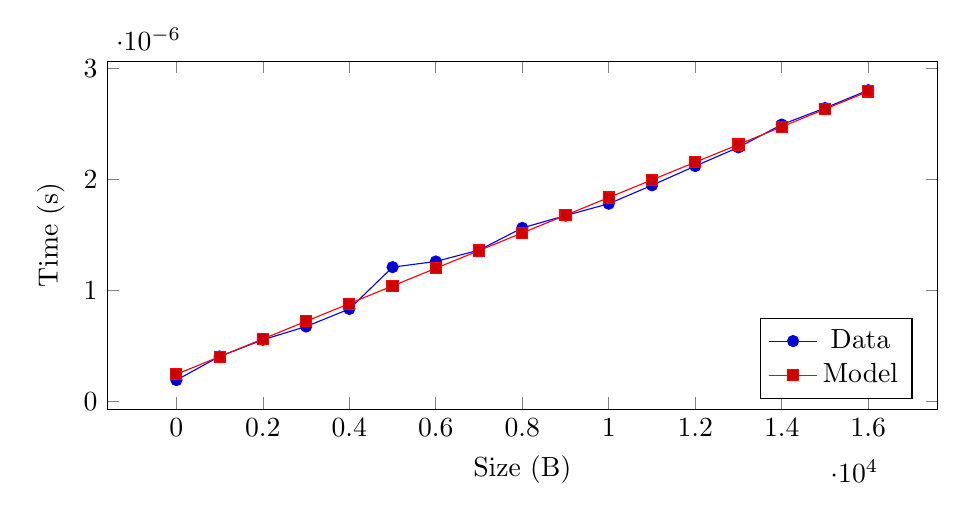
\begin{tikzpicture}
\begin{axis}[legend pos=south east,height=6cm,width=\textwidth,xlabel={Size (B)},ylabel={Time (s)}]
\addplot coordinates {
  (1,1.90705e-07)
  (1001,4.04215e-07)
  (2001,5.54506e-07)
  (3001,6.74211e-07)
  (4001,8.32396e-07)
  (5001,1.20983e-06)
  (6001,1.26129e-06)
  (7001,1.36371e-06)
  (8001,1.56382e-06)
  (9001,1.67521e-06)
  (10001,1.78203e-06)
  (11001,1.94837e-06)
  (12001,2.12196e-06)
  (13001,2.29048e-06)
  (14001,2.49609e-06)
  (15001,2.64557e-06)
  (16001,2.8065e-06)
};
\addlegendentry{Data}
\addplot coordinates {
  (1,2.42924e-07)
  (1001,4.02418e-07)
  (2001,5.61912e-07)
  (3001,7.21406e-07)
  (4001,8.809e-07)
  (5001,1.04039e-06)
  (6001,1.19989e-06)
  (7001,1.35938e-06)
  (8001,1.51888e-06)
  (9001,1.67837e-06)
  (10001,1.83786e-06)
  (11001,1.99736e-06)
  (12001,2.15685e-06)
  (13001,2.31635e-06)
  (14001,2.47584e-06)
  (15001,2.63533e-06)
  (16001,2.79483e-06)
};
\addlegendentry{Model}
\end{axis}
\end{tikzpicture} \\
$\alpha \approx $ {\tt 2.43e-07},
$\beta \approx $ {\tt 1.59e-10}

  \end{center}
\end{frame}


\begin{frame}
  \frametitle{Where we are now}

  Can write a lot of MPI code with 6 operations we've seen:
  \begin{itemize}
  \item {\tt MPI\_Init}
  \item {\tt MPI\_Finalize}
  \item {\tt MPI\_Comm\_size}
  \item {\tt MPI\_Comm\_rank}
  \item {\tt MPI\_Send}
  \item {\tt MPI\_Recv}
  \end{itemize}
  ... but there are sometimes better ways.
  
  \vspace{5mm}
  Next time: non-blocking and collective operations!
\end{frame}

\end{document}
